\paragraph{Fonctionnement}

Cette partie va illustrer ce rapport d'un jeux de copies d'�crans
rcapitulant les fonctionnalit�s implant�es.

La premi�re �tape � r�aliser est l'�criture de l'algorithme (voir
le Manuel d'utilisation) et sa compilation en bytecode Java.

L'�tape suivante est la cr�ation du graphe sur lequel la simulation va s'effectuer.

\begin{figure}[ht]
  \centering
  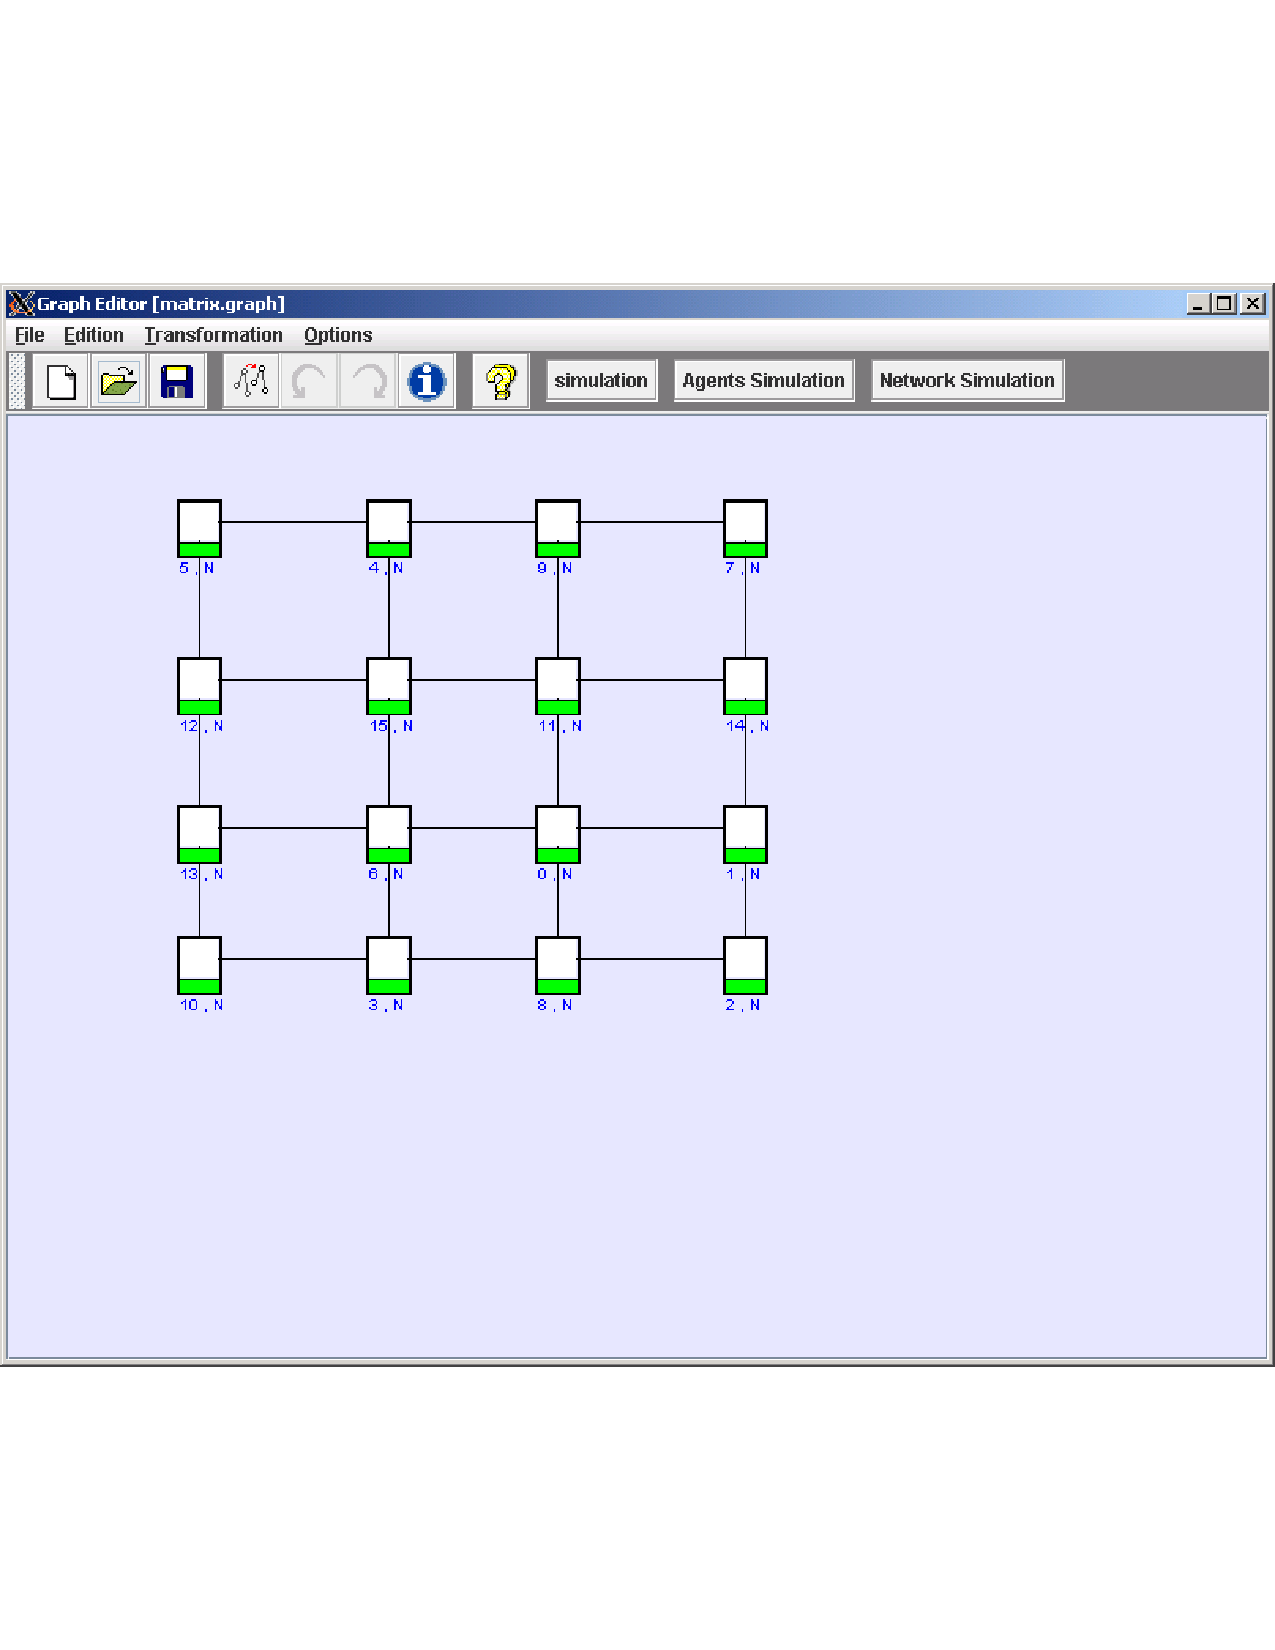
\includegraphics[width=10cm]{fonctionnement-matrix-graph}
  \caption{Fenetre d'edition d'un graph : une grille 4x4}
  \label{fig:fonctionnement-matrix-graph}
\end{figure}

Une fois fois le graphe cr��, la fenetre de simulation peut-etre
lanc�e. A cette �tape, nous ajoutons des agents sur des sommets de
d�part que l'on choisi par s�lection ou par algorithme.

\begin{figure}[ht]
  \centering
  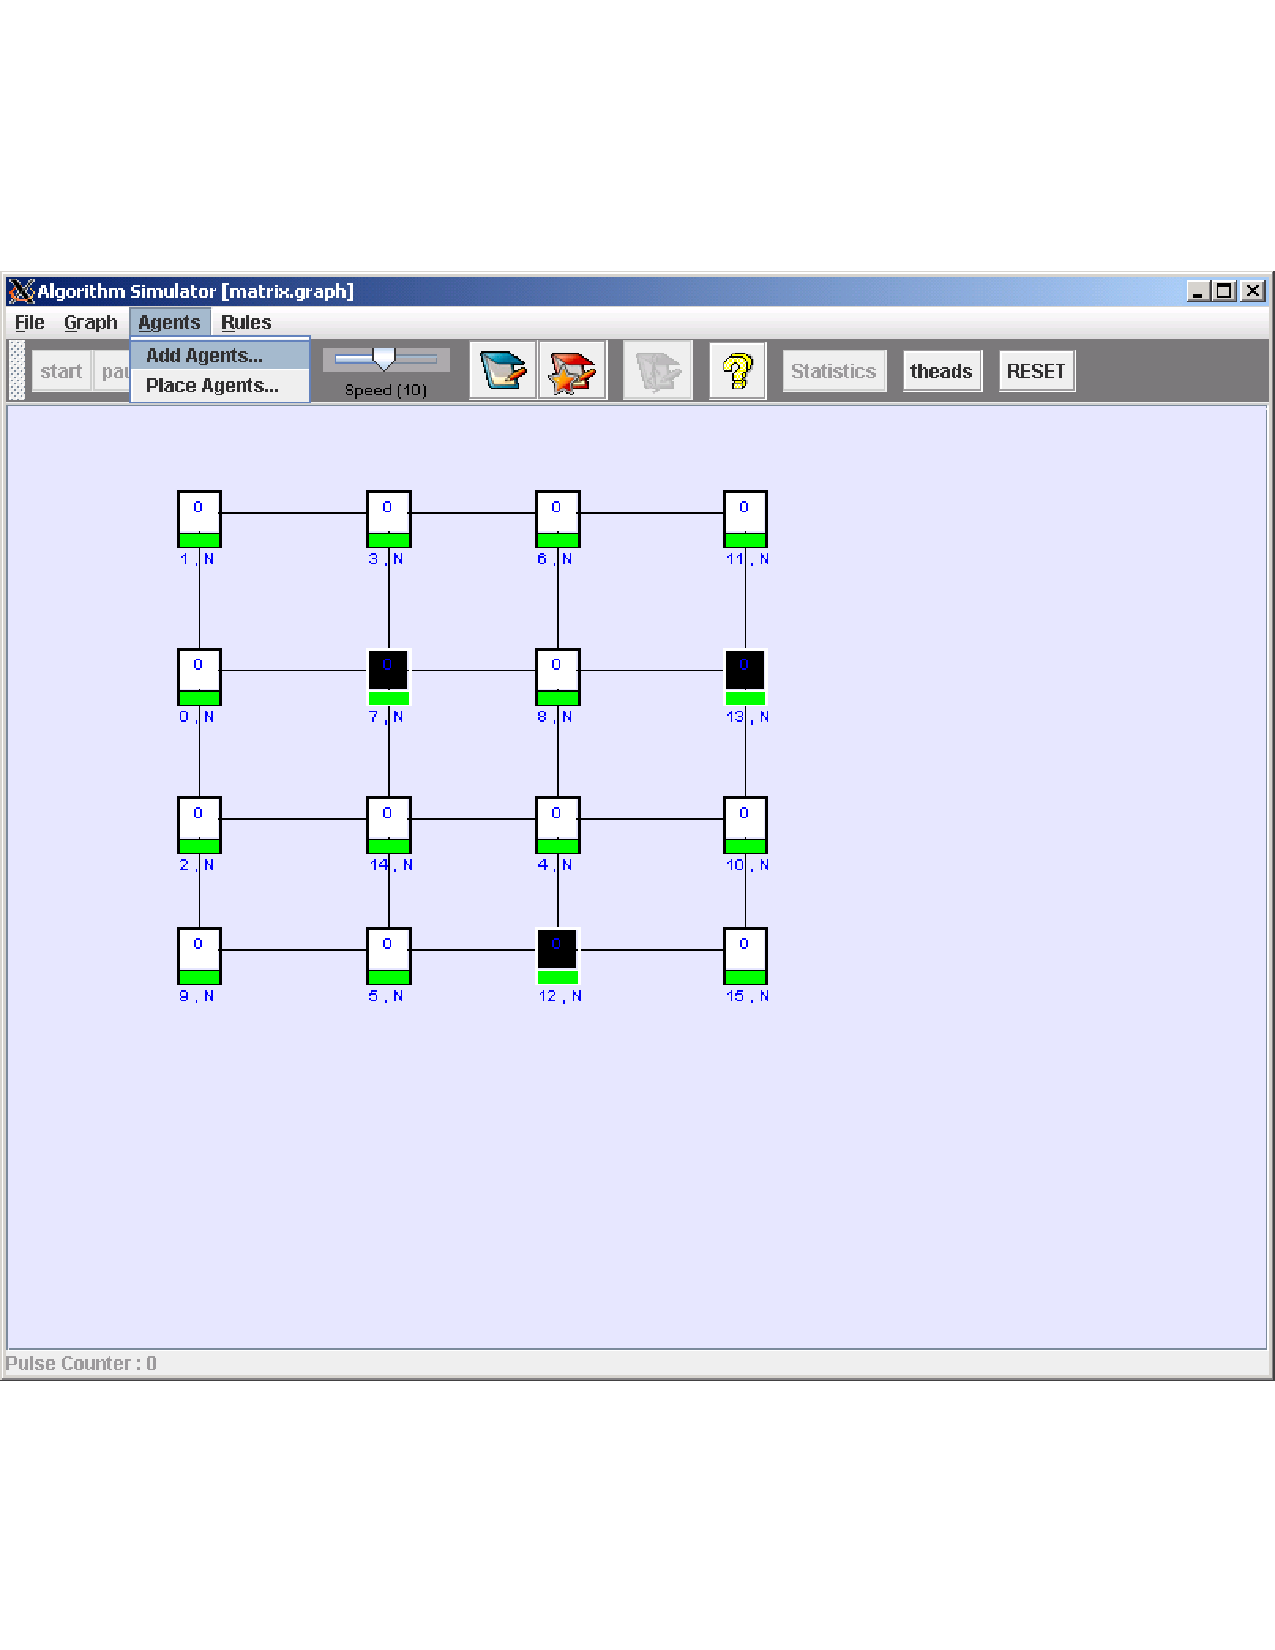
\includegraphics[width=10cm]{fonctionnement-ajout-agent}
  \caption{Ajout d'un type d'agent sur les trois sommets s�lectionn�s}
  \label{fig:fonctionnement-ajout-agent}
\end{figure}

La quatri�me �tape consiste � choisir notre agent compil� dans la
fenetre de s�lection.

\begin{figure}[ht]
  \centering
  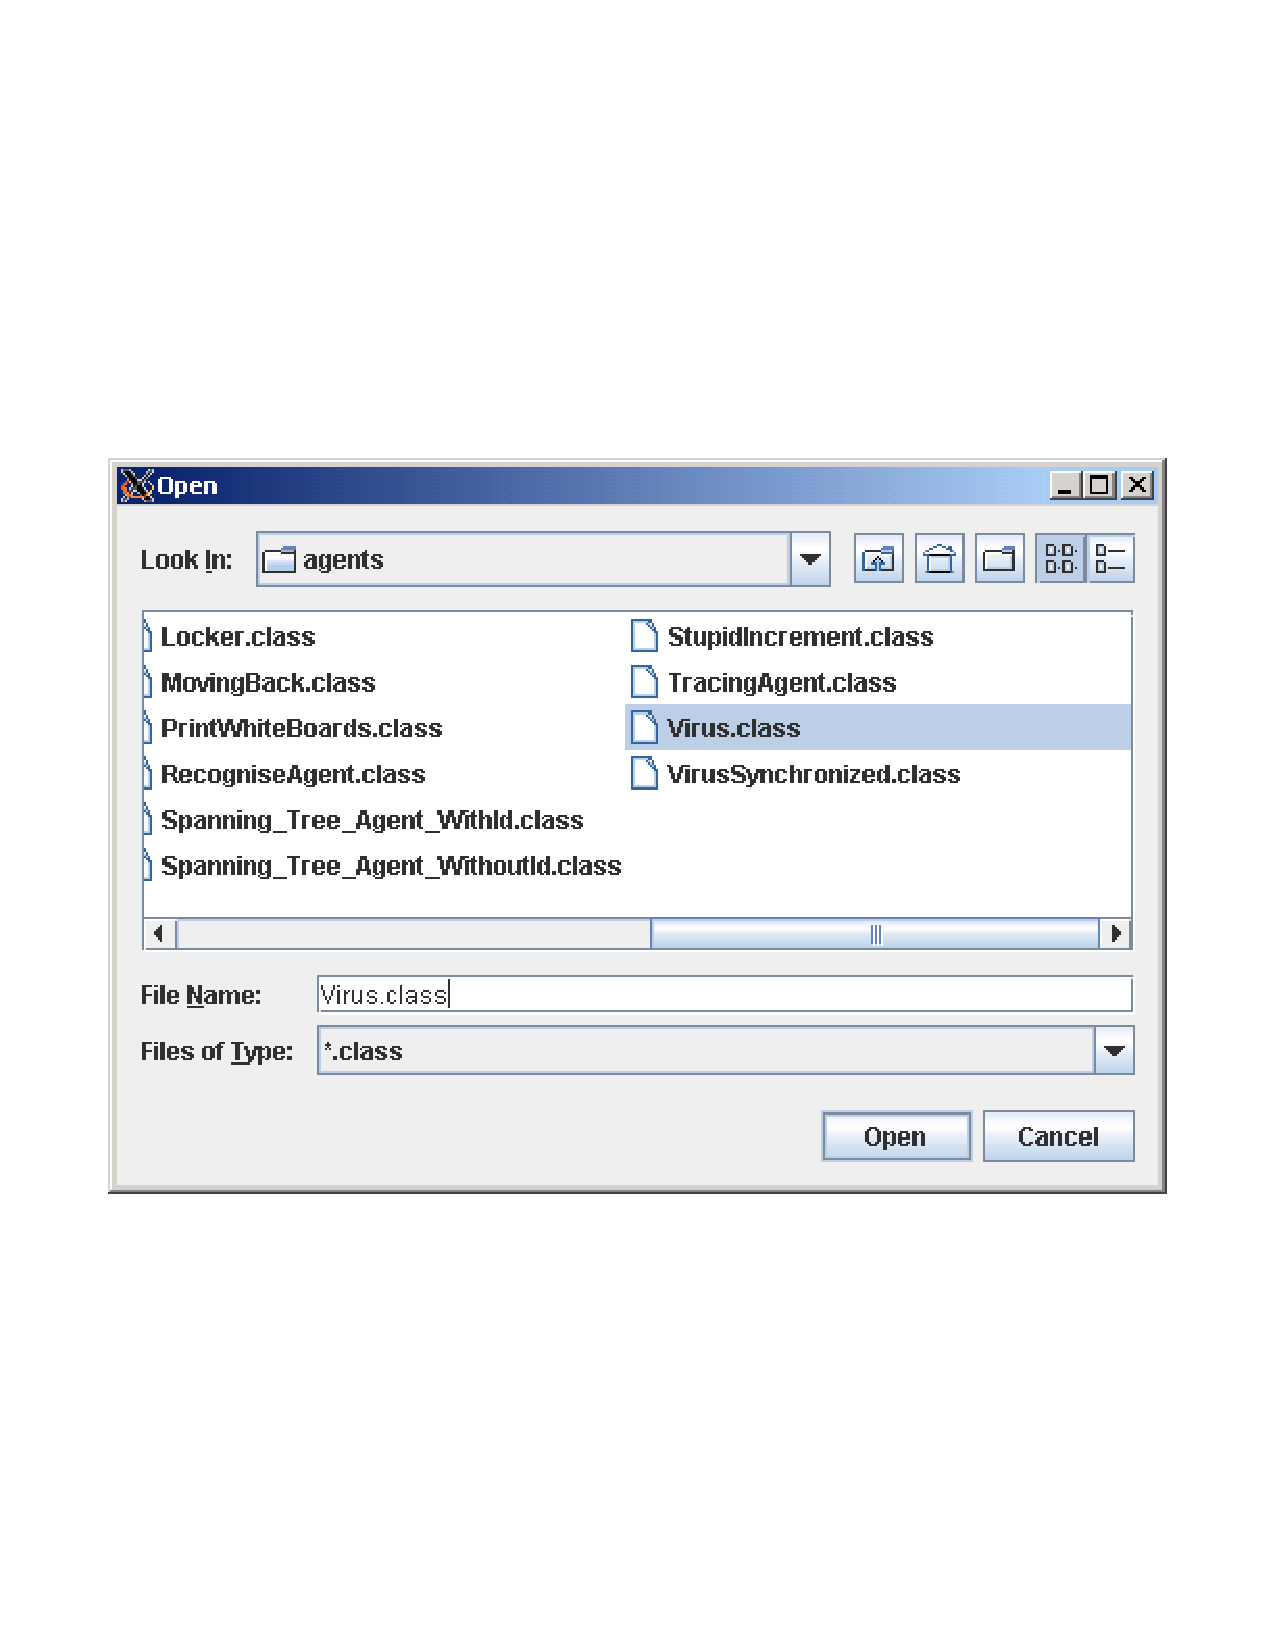
\includegraphics[width=10cm]{fonctionnement-choix-agents}
  \caption{Selection du type d'agent voulu}
  \label{fig:fonctionnement-choix-agents}
\end{figure}

Ensuite vient l'�tape de la simulation proprement dite. Les agents se
d�placent, marquent des aretes, se clonnent ou se suicident
conform�ment � ou aux l'algorithmes d'agent que l'on vient de
programmer. Ces actions sont repr�sent� graphiquement dans la fenetre
de simulation.

\begin{figure}[ht]
  \centering
  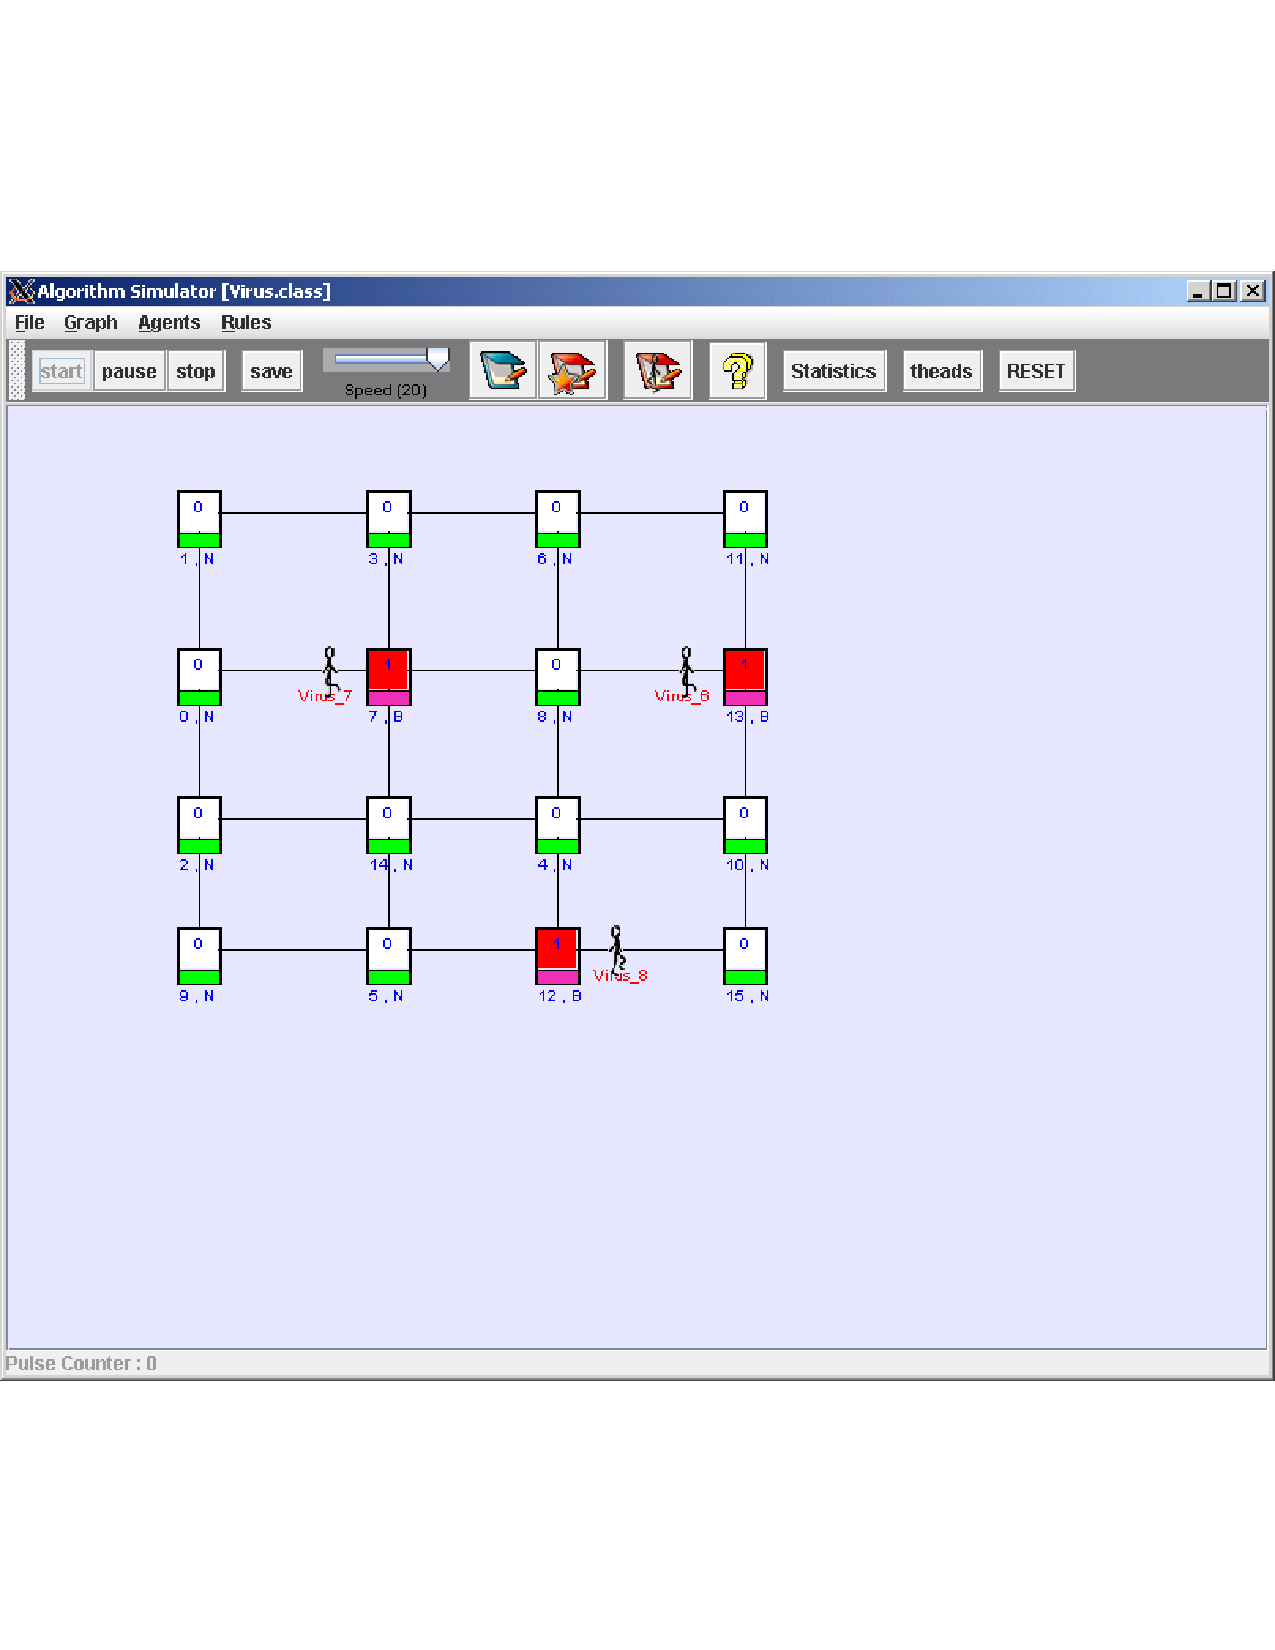
\includegraphics[width=10cm]{fonctionnement-simu1}
  \caption{Simulation en cours : les agents se d�placent sur le graph}
  \label{fig:fonctionnement-simu1}
\end{figure}

On peut �galement visualiser et �diter les whiteboards des agents et
des sommets au cours de la simulation en temps r�el.

\begin{figure}[ht]
  \centering
  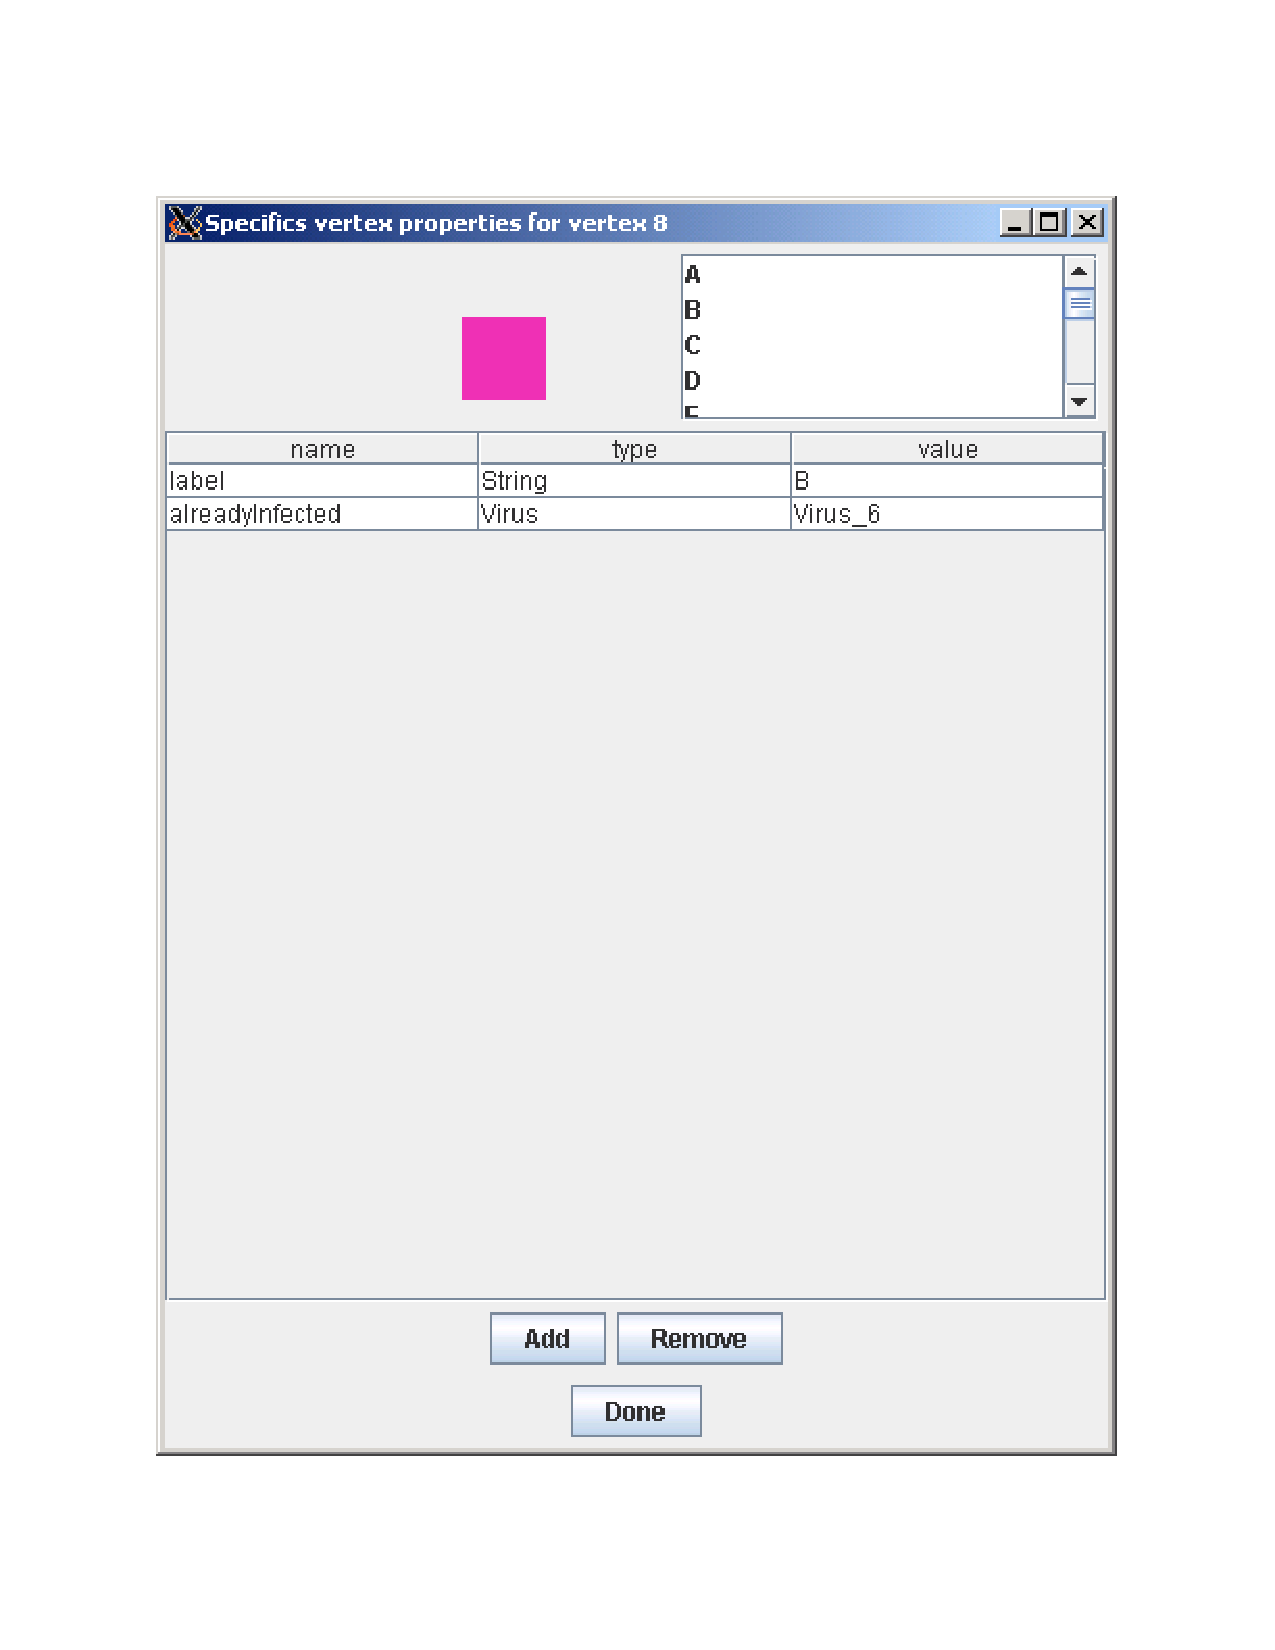
\includegraphics[width=10cm]{fonctionnement-vertex-properties}
  \caption{Visualtisation des informations du whiteboard d'un sommet}
  \label{fig:fonctionnement-vertex-properties}
\end{figure}

Lorsque tous les agents ont termin�s, la simulation se termine � son
tour et en informe l'utilisateur.

\begin{figure}[ht]
  \centering
  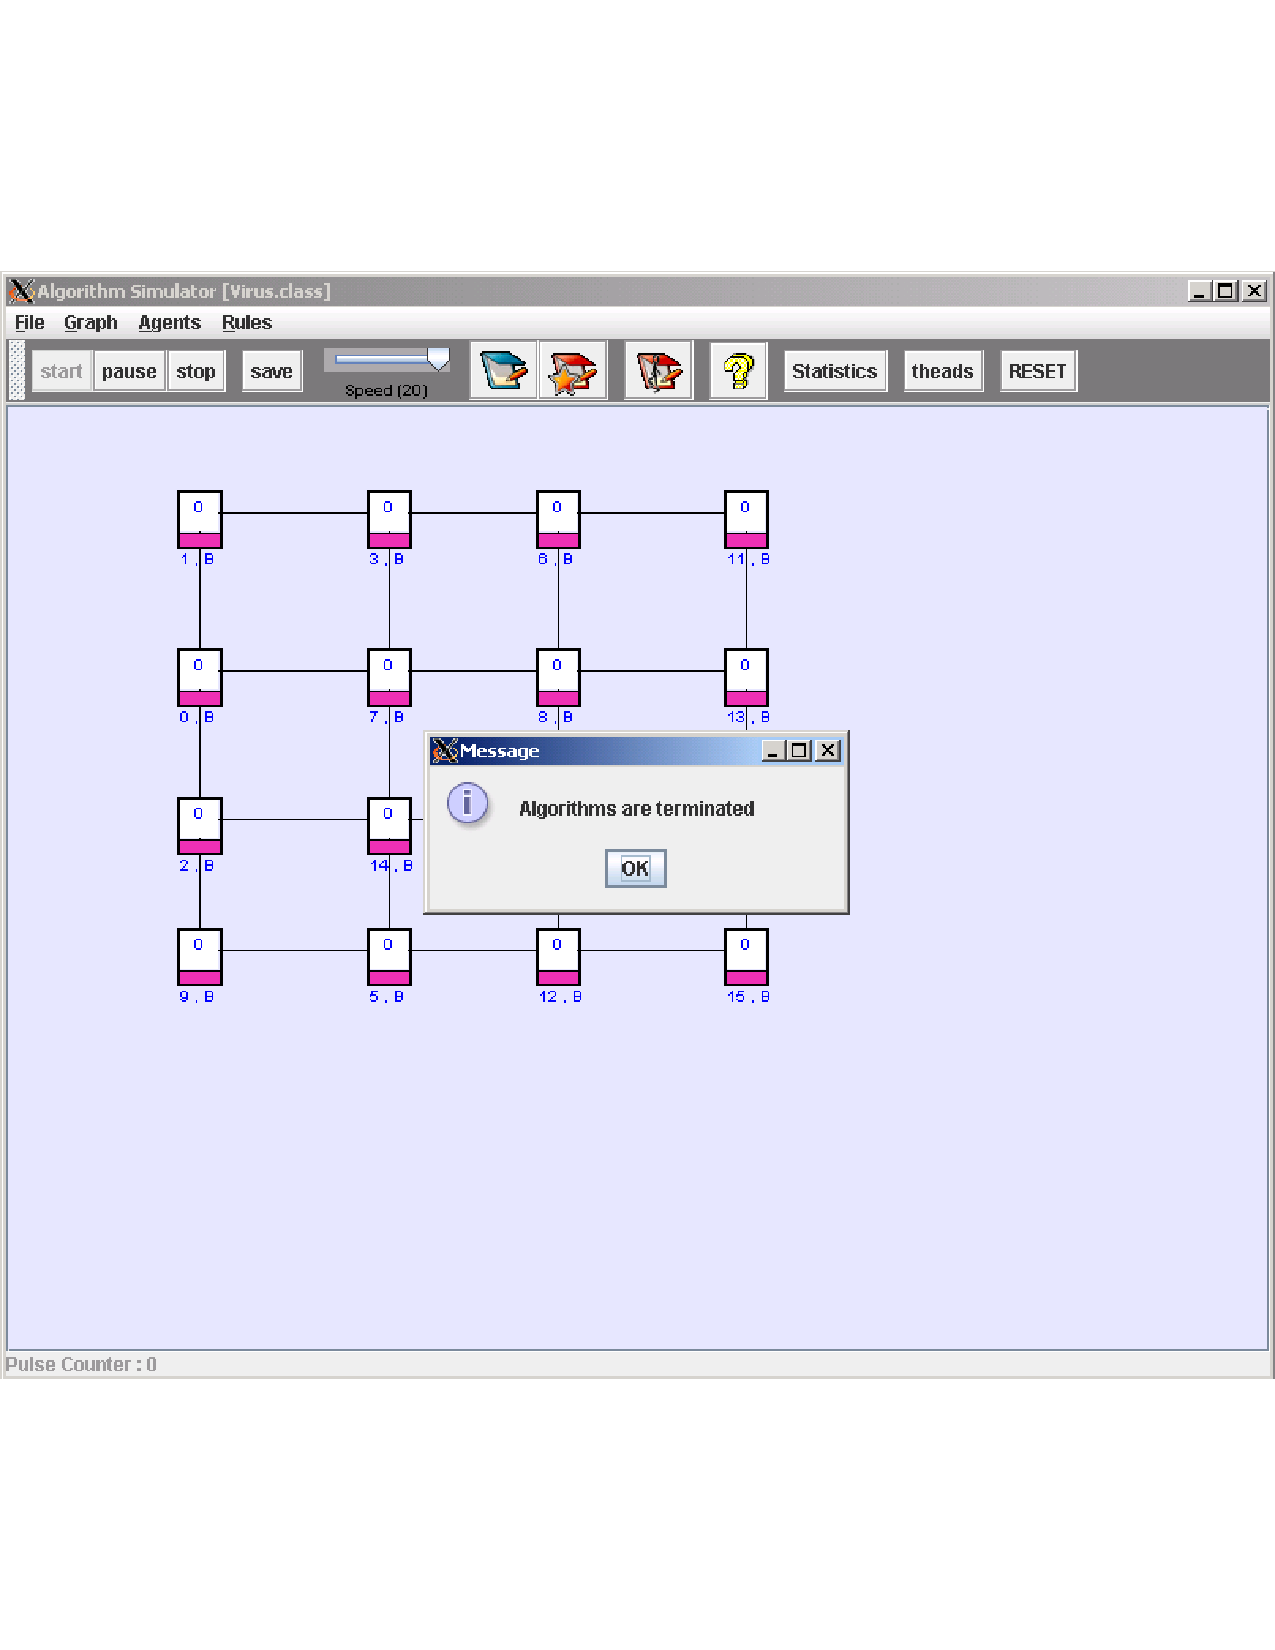
\includegraphics[width=10cm]{fonctionnement-simu-terminated}
  \caption{Les algorithmes sont termin�s, tous les agents sont mort}
  \label{fig:fonctionnement-simu-terminated}
\end{figure}

Des statistiques param�trables peuvent �galement etre �tablies. Pour
cela l'utilisateur doit avoir pr�alablement programm� sa classe de
calcul de statistiques et l'avoir compil� (voir le Manuel
d'utilisation).

\begin{figure}[ht]
  \centering
  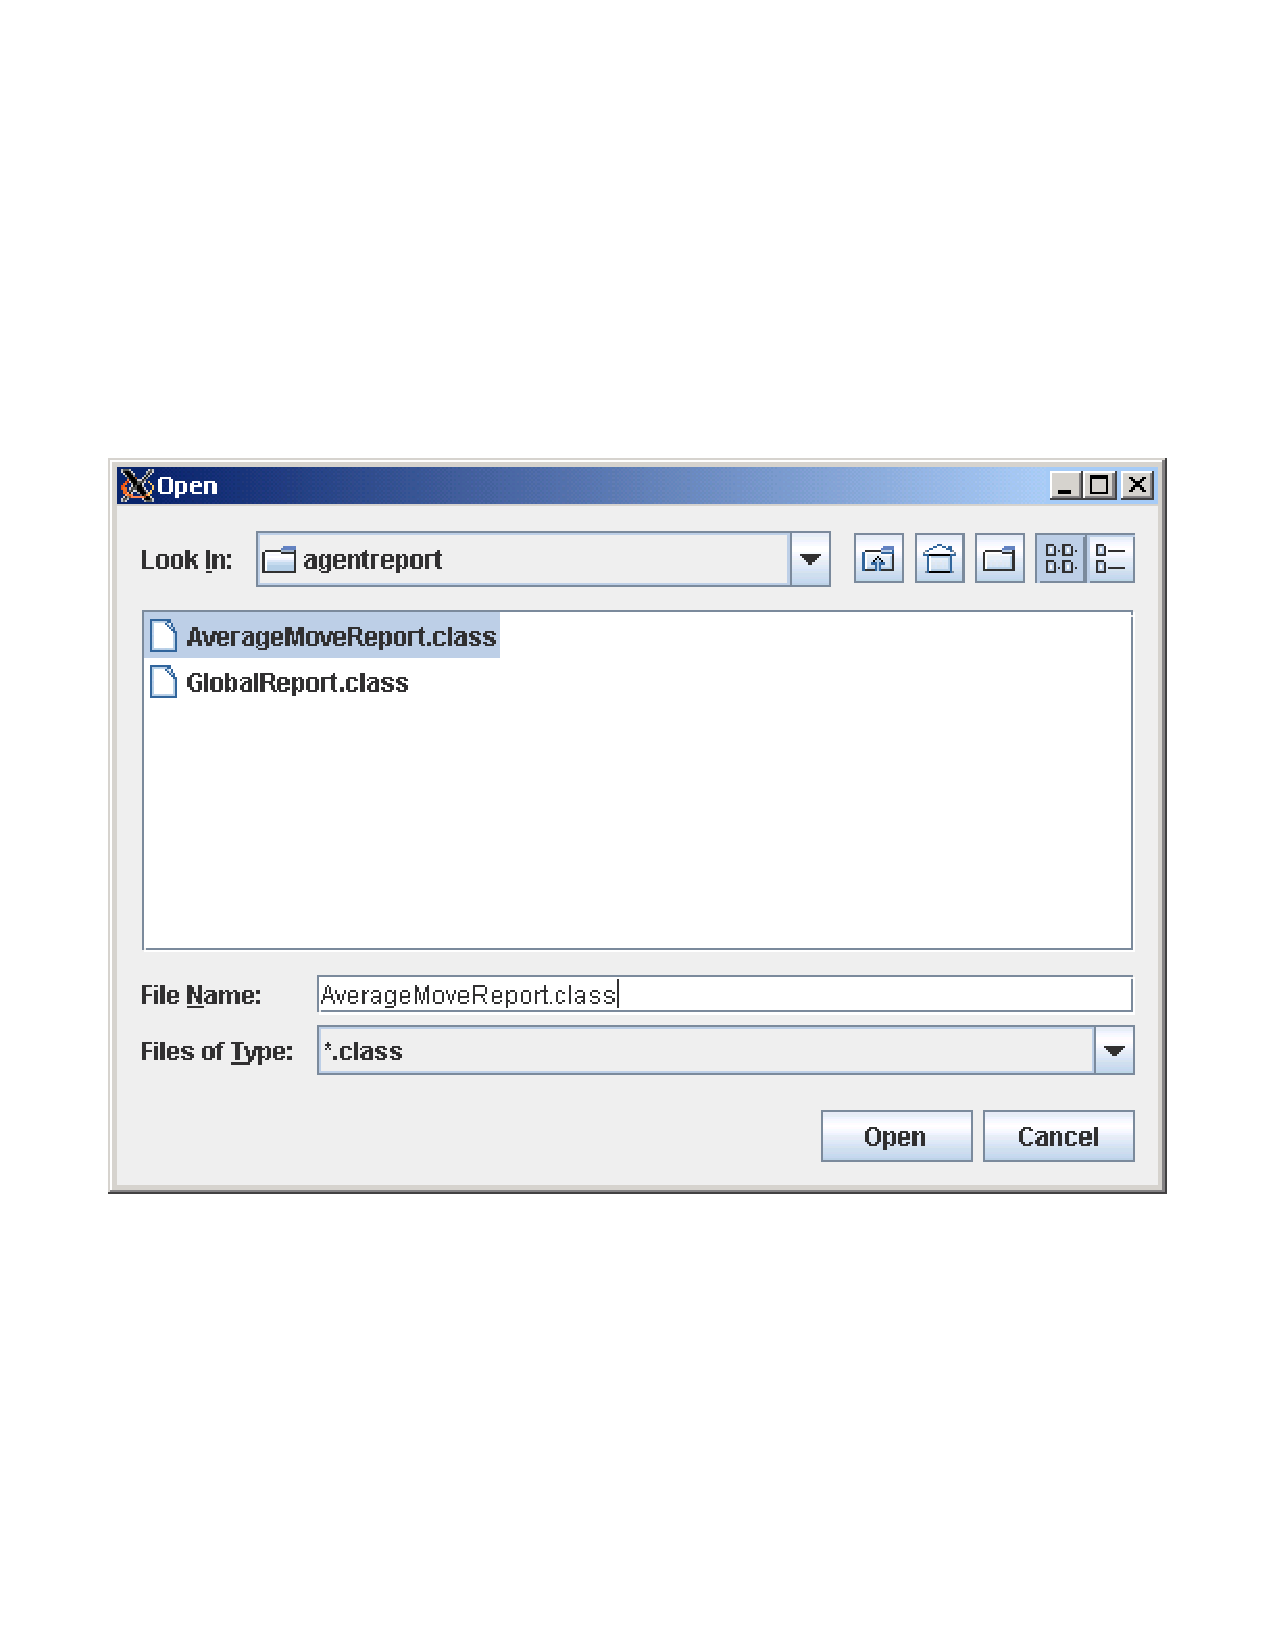
\includegraphics[width=10cm]{fonctionnement-choix-stats}
  \caption{Choix de la m�thode de calcul des satistiques}
  \label{fig:fonctionnement-choix-stats}
\end{figure}


\begin{figure}[ht]
  \centering
  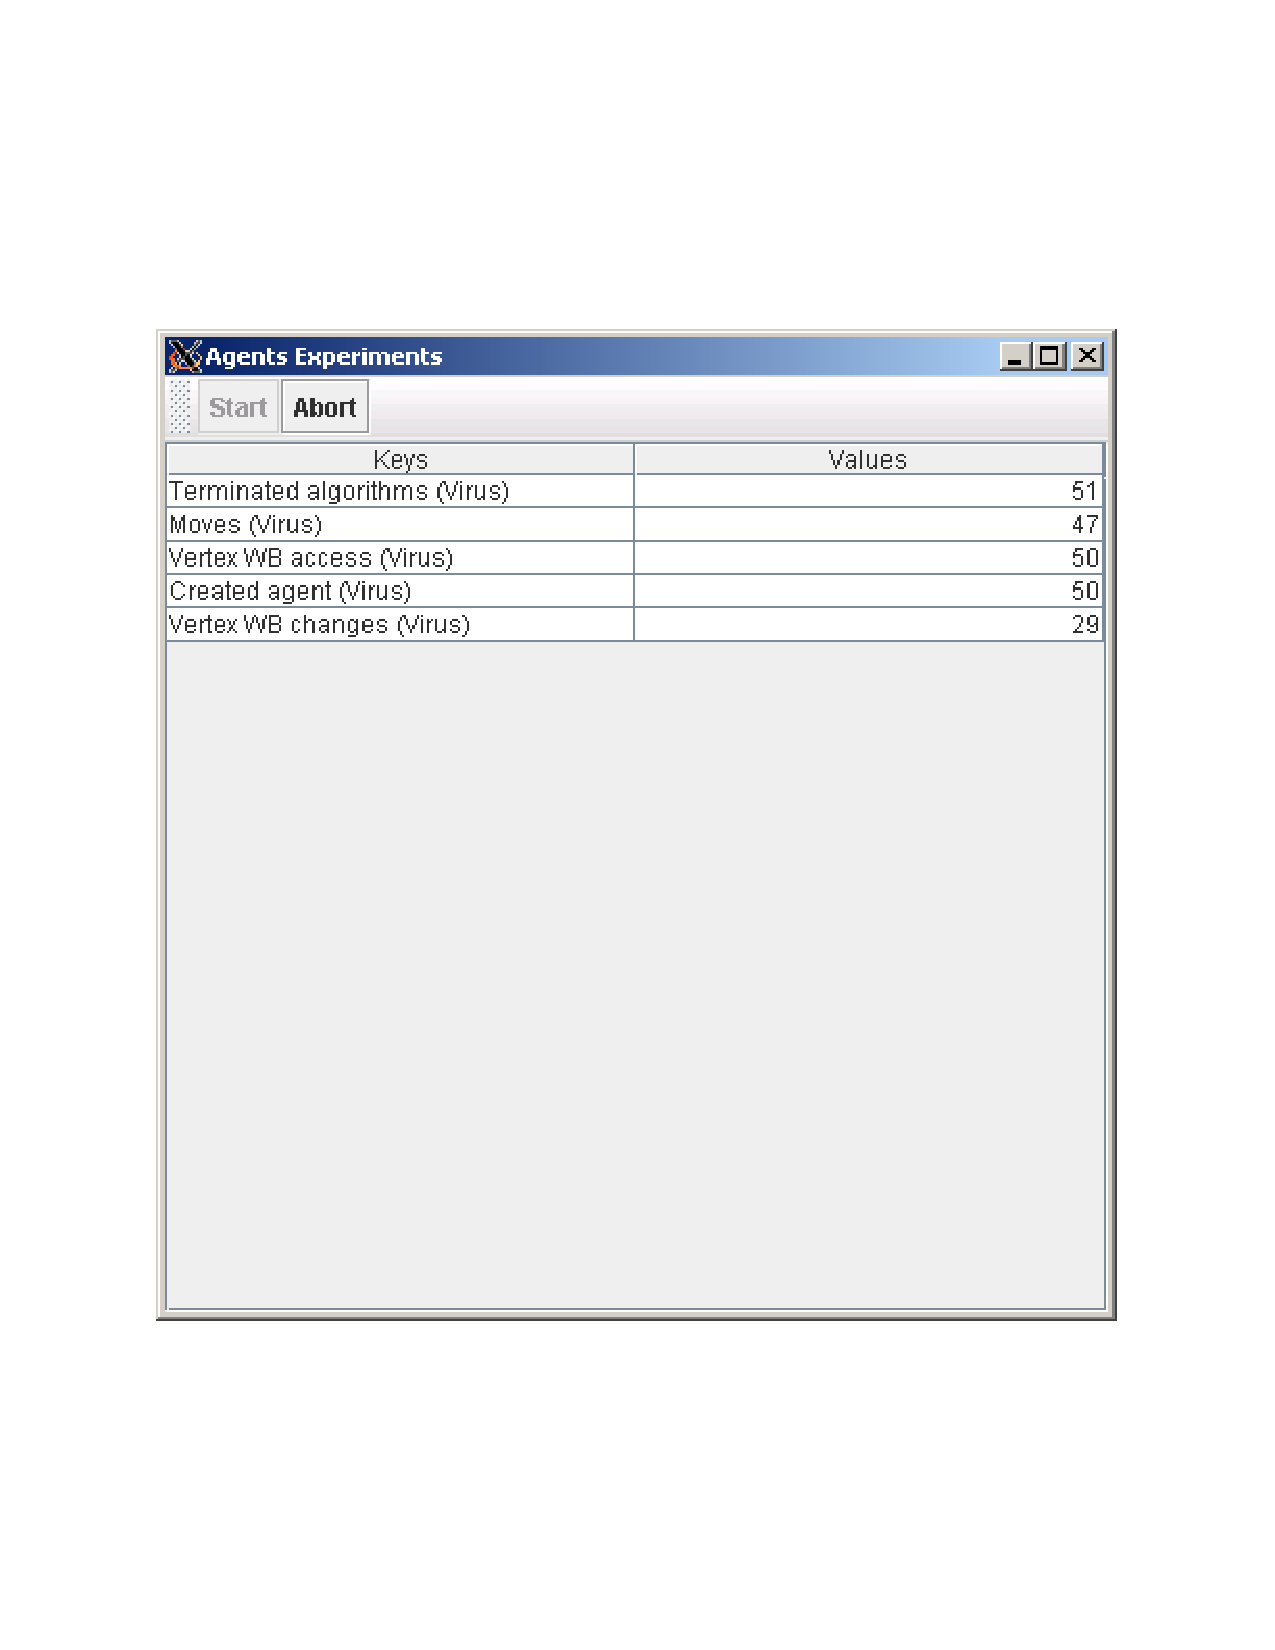
\includegraphics[width=10cm]{fonctionnement-stats}
  \caption{R�sultats du calcul de nos statistiques}
  \label{fig:}
\end{figure}



%\paragraph{Ecriture d'un algorithme}




%%% Local Variables: 
%%% mode: latex 
%%% TeX-master:  "rapport" 
%%% TeX-PDF-mode: t 
%%% coding:latin-1 
%%% End:
